\documentclass[a4paper, 12pt,twocolumn, french]{article}

\usepackage{babel}
\usepackage[T1]{fontenc}
\usepackage[utf8]{inputenc}
\usepackage{lmodern}

\usepackage{geometry}
\usepackage{graphicx}
\usepackage{tikz}

\newcommand*\circled[1]{
	\tikz[baseline=(char.base)]{
		\node[shape=circle,draw,inner sep=2pt] (char) {#1};
	}
}

% Define the margins
\geometry{top=2cm,left=2cm, right=2cm, bottom=2cm}

\title{Communications et Multi Agents}
\author{Guilhem \bsc{Marion} et Matthieu \bsc{Vieira}}
\date{juillet 2018}

\begin{document}

\maketitle

\section{Structure du programme}

Dans le cadre de l'UE Techniques de l'Intelligence Artificielle, nous avons construit un système multi-agents dont le but est, pour chaque agent, de se déplacer sur une grille à deux dimensions afin de rejoindre sa case objectif. Les agents sont dotés de capacités de raisonnement et de réactions indépendantes, ils sont capables de se déplacer sur la grille en même temps (multi-threading).

Notre programme, écrit en Python 3, est composé de deux fichiers :
\begin{description}
	\item[Puzzle.py] qui est le point de départ du programme, il génére les grilles et créé les agents.
	\item[Agent.py], qui implémente la classe \textit{thread} et instancie les agents étant donné ques les agents sont autonomes c'est ici que toutes les stratégies sont implémentées (déplacements et communications).
\end{description}

Chacun des agents est indépendant, et ce fait, agit comme un processus indépendant (thread), il y par conséquent des problèmes d'accès concurrents lors des mouvements, nous avons résolu ce problème très facilement en utilisant des techniques d'accès concurrents non bloquants. A l'initialisation une grille est constuire et les agents y sont placés aléatoirement, le nombre d'agent ainsi que la taille de grille peuvent être aisaiement changés. Veuillez vous référer au README.md ou à la vidéo pour les questions d'utilisation. 

Comme le principe des systèmes multi-agents est d'avoir un système autonome et non centralisé, nous avons jugé opportun de ne pas se limiter à des règles expertes de mouvement et résolution de cas pathologiques. Nous avons, bien entendu, défini des stratégies efficaces pour la résolution des principaux problèmes mais nous avons aussi ajouté de l'aléatoire dès que possible pour que les agents puisse sortir eux-même de situations délicates.

Nous avons lancé un script calculant le nombre de coups moyens pour toutes les configurations avec des tailles de grilles entre 3 et 10 avec un taux de remplissage d'agents de 40\%. Nous avons observé un nombre de coups moyens très compétitifs et un poucentage d'échec (temps de traitment trop long) de moins de 3\%.


Dans la suite de ce rapport, nous prendrons pour chaque exemple une grille de taille $n \times n$ avec $n = 5$.

\section{Construction des cas}

\subsection{Le cas à un agent}

\begin{figure}[h]
	\centering
	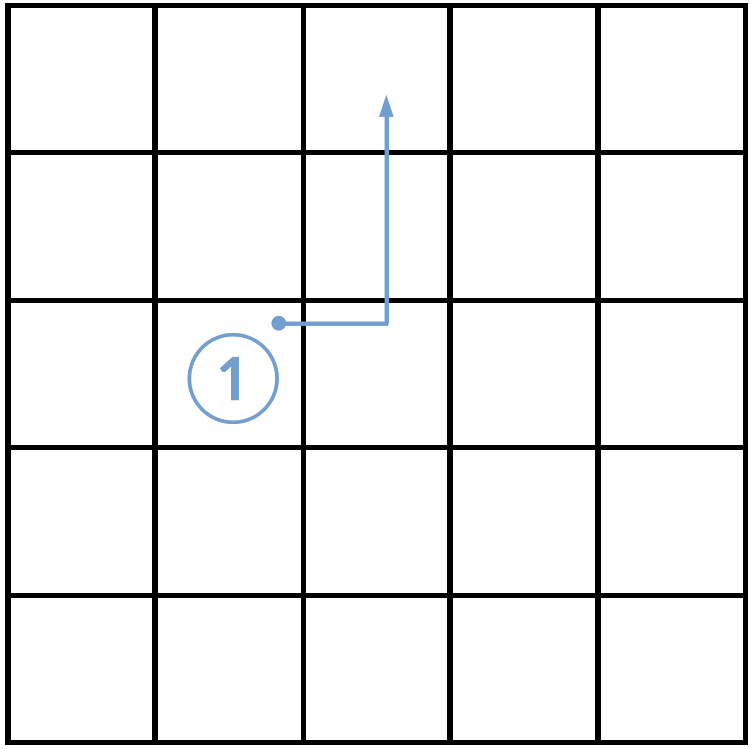
\includegraphics[width=150px]{images/base_case.png}
	\caption{Cas à 1 agent rejoingnant son objectif.}
\end{figure}

C’est le cas le plus simple du programme. L'agent est seul sur la grille et a un objectif. Tant qu'il n'est pas sur sa case d'arrivée, l'agent calcule la distance par rapport à celle-ci pour chacune des cases sur lesquelles il peut se déplacer. Dans le cas d'un quadrillage comme ici, la distance de Manhattan, donnée par la formule ci-dessous, est plus adaptée que la classique distance euclidienne.

\[
d(a, b) = |x_a - x_b| + |y_b - y_a|
\]


Dans le cas où deux directions ont la même distance Manhattan, on choisit aléatoirement une des deux directions.

\begin{figure}[h]
	\centering
	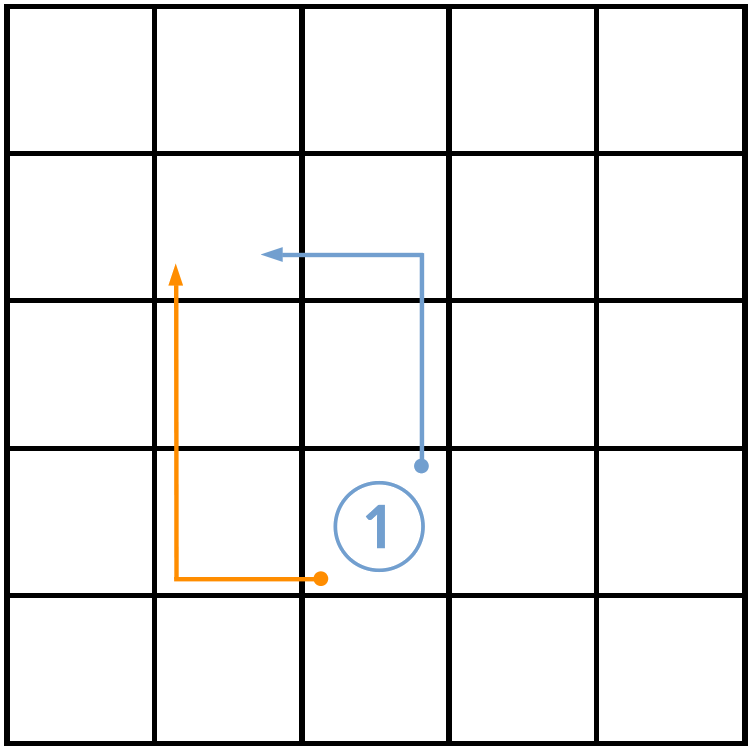
\includegraphics[width=150px]{images/manhattan_equal.png}
	\caption{Exemple de distances de Manhattan égales.}
\end{figure}

Le cas à un agent ne présente aucun bloquage possible : l'agent arrive forcément sur sa case objectif, en empruntant le plus court chemin.

\subsection{Le cas à deux agents}

A partir de deux agents il faut prendre en compte les eventuels bloquages, pour cela si un agent est bloqué par un autre dans son déplacement il lui envoie un message lui demandant de se déplacer, si celui-ci est sur sa case objectif ou a un mouvement opposé au premier agent il se déplace orthogonalement au déplacement du premier agent et attend que celui-ci se déplace pour rejoindre sa place. Si l'agent n'est si sur sa case objectif ni en mouvment opposé au premier agent il faut juste attendre qu'il fasse un mouvement pour rejoindre sa case objectif et ainsi liberer la case.

\begin{figure}[h]
	\centering
	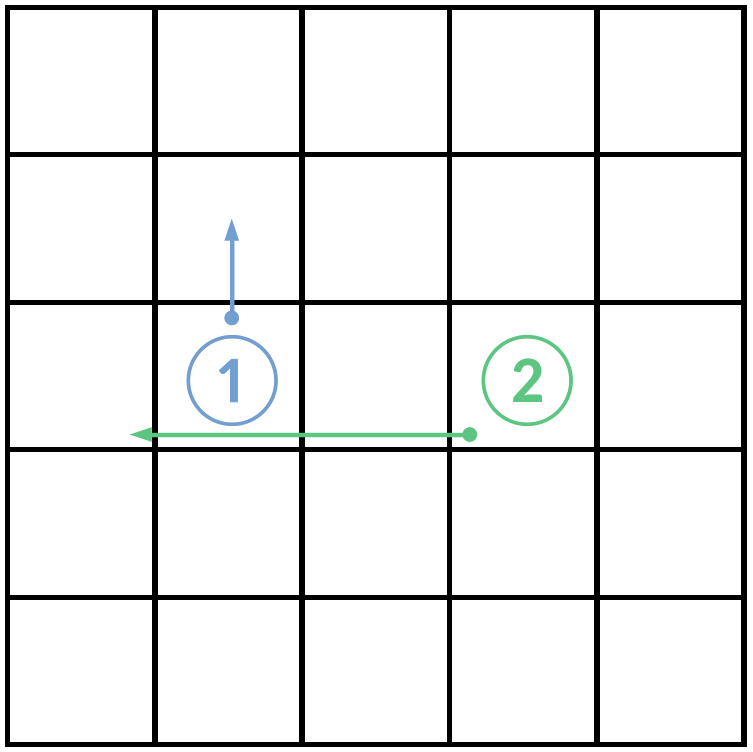
\includegraphics[width=150px]{images/2_agents.png}
	\caption{Cas à deux agents.}
\end{figure}


\begin{figure}[h]
	\centering
	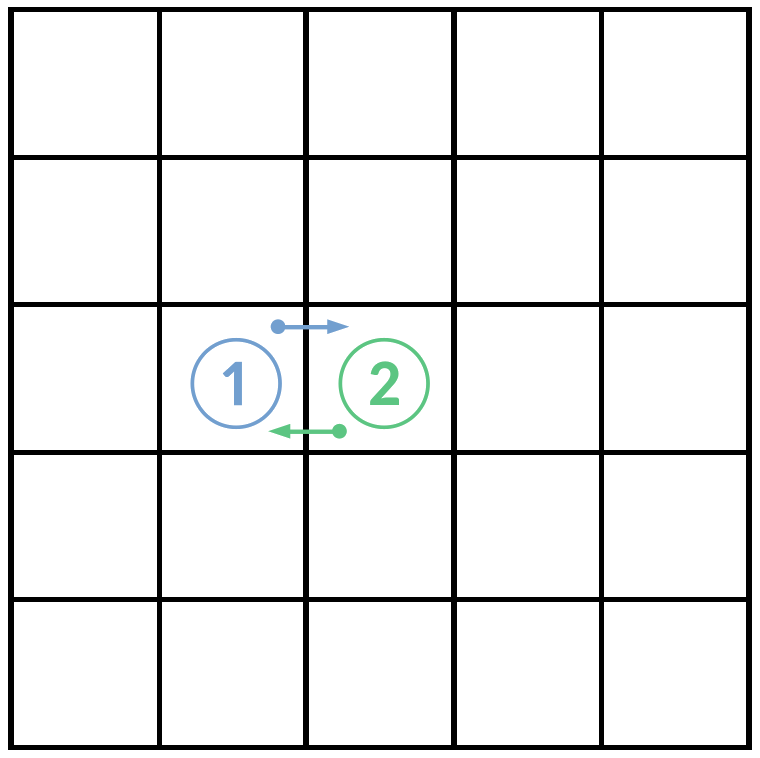
\includegraphics[width=150px]{images/switch.png}
	\caption{Exemple du cas où deux agents ont des directions opposées.}
\end{figure}

La situation décrite dans la figure 3 explique le cas où deux agents ont des directions opposées. L'agent \circled{1} souhaite se rendre sur la case située à droite de l'agent \circled{2} qui lui veut aller sur la case occupée par l'agent \circled{1}. Les deux agents s'envoyant des messages contradictoires, l'un va comprendre qu'il doit effectuer un mouvement orthogonal par rapport à l'autre agent afin de le laisser passer pour ensuite continuer son chemin.


\subsection{Le cas à trois agents}

Dans cette situation, on peut faire face à un nouveau cas pathologique.

\begin{figure}[h]
	\centering
	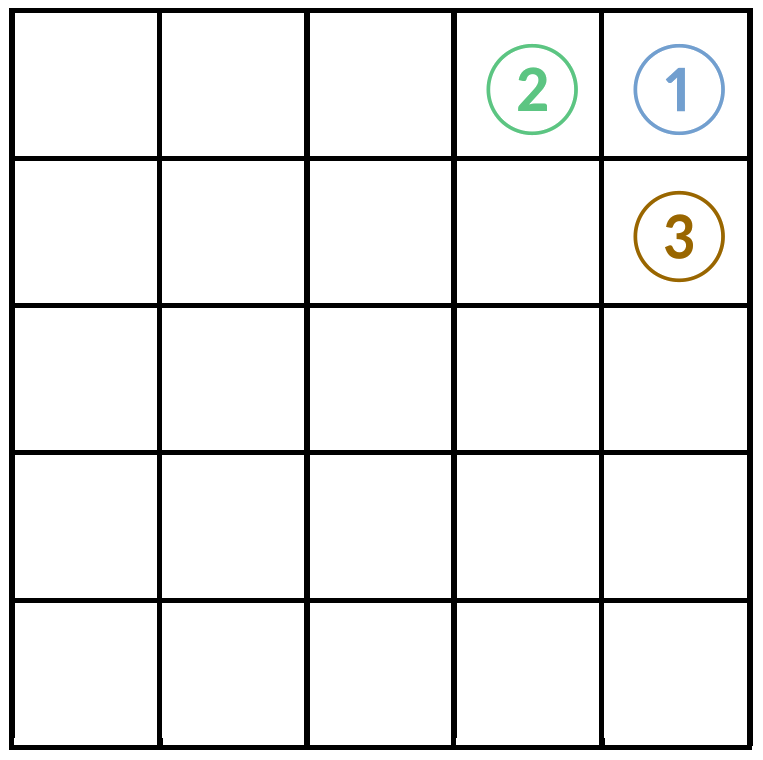
\includegraphics[width=150px]{images/3_agents.png}
	\caption{Cas à trois agents.}
\end{figure}

L’agent \circled{1} n'est pas sur sa case d'objectif et est ici \og{} enfermé \fg{} : il n'a aucun mouvement possible, c'est pourquoi il envoie un message à tous ses voisins pour leur demander de bouger.

\subsection{Le cas à quatre agents}

\begin{figure}[h]
	\centering
	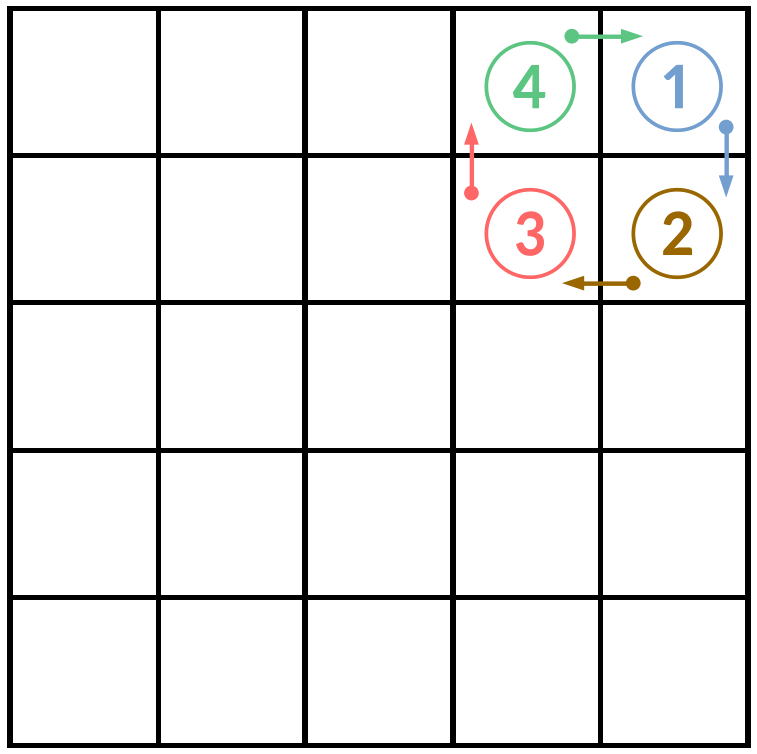
\includegraphics[width=150px]{images/4_agents.png}
	\caption{Cas à quattre agents.}
\end{figure}

Nous faisons désormais face à un cycle où chaque agent $i$ souhaite aller sur la case occupée par l'agent $i + 1$, qui est en réalité une généralisation du cas évoqué plus haut pour deux agents qui souhaitent aller dans des directions opposées en se \og{} croisant \fg{}. La résolution se fait de la même manière : un des agents va prendre la décision d'effectuer un mouvement orthogonal pour \og{} sortir du carré \fg{} et permettre au système de se résoudre.

\subsection{Le cas à cinq agents}

Le dernier cas pathologique présenté ci-dessous se déroule sur une grille avec 5 agents, mais ressemble quelque peu au cas pathologique avec deux agents. Les agents \circled{2}, \circled{3} et \circled{5} sont à leur case d'objectif et ne souhaitent donc pas bouger. Les agents \circled{1} et \circled{4} doivent \og{} intervertir \fg{} leurs places mais aucun ne peut effectuer un mouvement orthogonal, et se contentent de \og{} monter \fg{} et \og{} descendre \fg{}. Au bout d'un certain temps, voyant que rien ne progresse, un des agents va alors effectuer un nombre de mouvements aléatoires défini par la constante \texttt{RANDOM\_MOVE}. Cela va permettre de suffisamment l'éloigner de la situation bloquée pour qu'il trouve un autre chemin dans la grille.

Nous pensons que la plupart des cas pathologiques sont résolus avec cette technique, des hyper-paramètres sont présents en haut du fichier \textit{Agent.py} qui peuvent être tweakés afin de diminuer le nombre de \textit{fails} ou réduire le nombre de coups moyens. Nous n'avons que trop peu joué avec ces paramètres, avec un peu plus de temps et de la puissance de calcul il faudrait apprendre statistiquement ces hyper-paramètres afin de minimiser le nombre de coups moyen. 

\begin{figure}[h]
	\centering
	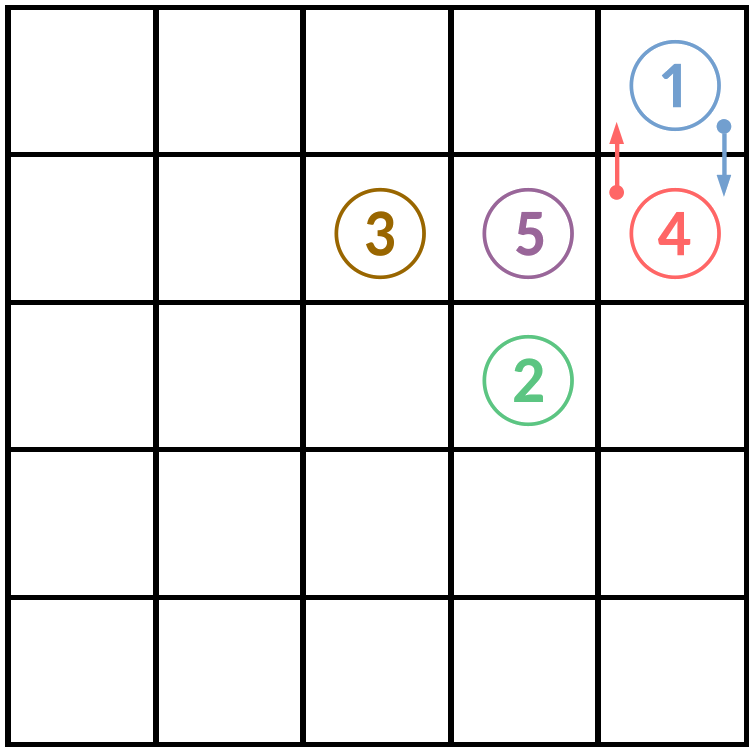
\includegraphics[width=150px]{images/5_agents.png}
	\caption{Résolution bloquage 5 agents.}
\end{figure}

\section{Conclusion}

Ce projet nous a permi de nous confronté aux problèmes des systèmes multi-agents, la communication entre les agents et le test de l'efficacité de ces systèmes. Nous avons pris l'initiative de construire une système autonome dans le sens où l'agent d'aléatoire permet de résoudre des problèmes sans connaissance préalable dudit problème. 
Nous pensons avoir résolu relativement efficacement ce système mais il serait néanmoins pertinent de tweaker les hyper-paramètres, nottament concernant l'aléaoire, afin d'optimiser encore la résolution.

\end{document}
